%=============================================================================
% IEEEtran conference manuscript.
% Compile:  pdflatex ieee_calmnet.tex  (twice, for references)
%
% Every number in this file is traceable to a JSON in ../results/.
% Where two numbers exist for the same model they are BOTH reported and the
% reason for the difference is stated, rather than the better one being chosen.
%=============================================================================
\documentclass[conference]{IEEEtran}
\IEEEoverridecommandlockouts

\usepackage{cite}
\usepackage{amsmath,amssymb}
\usepackage{graphicx}
\usepackage{booktabs}
\usepackage{url}
\usepackage[hidelinks]{hyperref}

\begin{document}

\title{A Parameter-Efficient EEG Decoder with In-Network Session Adaptation,
Calibration and Abstention for Lower-Limb Exoskeleton Control}

\author{%
\IEEEauthorblockN{Esm E Moula Chowdhury Abha, Md Wahiduzzaman Suva,
and Muhammad Hasibur Rashid Chayon}
\IEEEauthorblockA{Department of Computer Science\\
American International University-Bangladesh, Dhaka, Bangladesh\\
Email: 26-94089-2@student.aiub.edu, 26-94088-2@student.aiub.edu,
chayon@aiub.edu}}

\maketitle

%-----------------------------------------------------------------------------
\begin{abstract}
Decoding walk/stop intent from scalp EEG for lower-limb exoskeleton control
requires more than per-epoch accuracy: the decoder is fitted once and must keep
working weeks later, a false Walk command moves a person's legs, and a decoder
that is uncertain should be able to decline. We present an architecture that
addresses all three inside the network. A label-free adaptive alignment layer
maintains a running spatial covariance and whitens by it at inference; a
multi-scale power stem preserves log-power ratios across three temporal
resolutions; and a selective head emits an abstention decision under a coverage
constraint.

The result is the most compact decoder in our comparison by a factor of two.
At \textbf{24\,181 parameters} it reaches 0.901 balanced accuracy on a
7-subject, 9-session longitudinal exoskeleton cohort --- within 0.012 of the
strongest published baseline evaluated in the same harness while using 53\,\% of
its parameters and 5\,\% of a transformer decoder's --- and it is the only model
in the comparison that also emits calibrated confidence (ECE 0.039) and a trained
abstention operating point (0.876 accuracy at 90\,\% coverage). Its alignment
layer removes 52\,\% and 84\,\% of session-to-session covariance drift on two
independent cohorts, in \textbf{15 of 15 subjects} ($p \le 10^{-4}$), against a
no-op control that shows no reduction. On the primary cohort the layer is
necessary rather than additive: with it removed, every remaining module together
contributes less than the measurement noise.

External validation on an independent treadmill cohort establishes the
architecture's operating envelope, and yields the result we consider most
transferable. In-network adaptation has a failure mode its offline counterpart
cannot have: the running estimate tracks whatever is currently streaming, so
under a protocol that presents classes in long contiguous blocks the layer
whitens away the class itself. We predict the threshold from the protocol,
observe it where predicted --- slowing adaptation past the class-block length
recovers 0.090 to 0.098 on every arm that uses alignment and exactly 0.000 on
both arms that do not --- and show the condition is \textbf{two-sided}: the rate
must be fast enough to track drift and slow enough not to track class, with the
two cohorts' optima opposite and each losing 0.06--0.09 at the other's setting.
Where class blocks outlast the drift timescale no admissible rate exists. Both
timescales are computable from the recording protocol before a model is fitted,
making this a design-time check rather than a post-hoc diagnosis.
\end{abstract}

\begin{IEEEkeywords}
brain--computer interface, EEG, test-time adaptation, covariate shift, selective
prediction, calibration, lower-limb exoskeleton
\end{IEEEkeywords}

%-----------------------------------------------------------------------------
\section{Introduction}

A brain--computer interface that drives a powered exoskeleton is not well
described by per-epoch classification accuracy alone. Three properties of the
deployment matter as much as the mean score.

\textbf{Longitudinal drift.} The decoder is fitted once and must keep working
weeks later. In our primary cohort this is literal: the model is fitted on
sessions 1--3 and tested on sessions 4--9, recorded across weeks. Electrode
montage, impedance and skin contact all change between sessions, shifting the
second-order statistics of the signal that any spatial filter depends on.

\textbf{Asymmetric cost.} A false Walk command moves a person's legs. Balanced
accuracy scores that identically to a missed Walk, and cannot distinguish one
long false activation from fifty scattered false windows. The quantity a wearer
experiences is spurious activations per minute of standing.

\textbf{No option to decline.} A classifier trained only for accuracy must emit a
decision for every window. A device acting on a confidence value needs that value
to mean something, and needs a principled way to do nothing when the evidence is
weak.

We address all three inside the network rather than in pre- or post-processing,
and evaluate on two independent cohorts. Our contributions are:

\begin{enumerate}
\item A compact architecture (24\,181 parameters) combining label-free in-network
      session adaptation, a ratio-preserving multi-scale power stem, and a
      selective head, reaching competitive accuracy with calibration and
      abstention that the baselines do not provide.
\item A validated drift mechanism: 52\,\% and 84\,\% reduction in
      session-to-session covariance distance across two cohorts, in every
      subject, against a no-op control that shares every code path.
\item A design condition for in-network adaptation --- the adaptation rate must
      exceed the class-block timescale and stay below the drift timescale ---
      demonstrated with a predicted threshold, a five-arm controlled sweep, and
      two exact null controls.
\item An external validation that fails, reported in full: the architecture does
      not transfer to the second cohort, and we identify why.
\end{enumerate}

%-----------------------------------------------------------------------------
\section{Related Work}

\textbf{Convolutional decoders.} ShallowFBCSPNet and Deep4Net~\cite{schirrmeister}
established the $\mathrm{square} \rightarrow \mathrm{pool} \rightarrow \log$
pipeline that our power stem descends from; EEGNet~\cite{lawhern} introduced the
depthwise--separable formulation that makes compact EEG decoders practical.
EEGNeX~\cite{eegnex} is a recent refinement of that family.

\textbf{Attention decoders.} ATCNet~\cite{atcnet} combines convolutional feature
extraction with temporal convolution and multi-head attention and is, in our
hands, the strongest baseline on the primary cohort. EEG
Conformer~\cite{conformer} pairs a ShallowFBCSP-style stem with a transformer
encoder; we note explicitly that this combination is already published, and an
independent implementation of it in our harness reproduced its score rather than
improving on it (0.848 against 0.843).

\textbf{Alignment and transfer.} Euclidean Alignment~\cite{hewu} whitens each
recording by the inverse square root of its mean covariance and is normally
applied offline in preprocessing; Riemannian transfer
methods~\cite{barachant,zanini} generalise this to the SPD manifold. Our
contribution is not the transform but making it an in-network layer that adapts
at inference without labels --- and the finding that doing so introduces a
failure mode the offline version cannot have.

\textbf{Epoch-sequence modelling} is standard in automatic sleep
staging~\cite{seqsleepnet,xsleepnet}. Our cross-epoch pathway transfers that idea
to intent decoding.

\textbf{Selective prediction.} The abstention head follows
SelectiveNet~\cite{selectivenet}, used as published.

%-----------------------------------------------------------------------------
\section{Method}

\begin{figure*}[t]
\centering
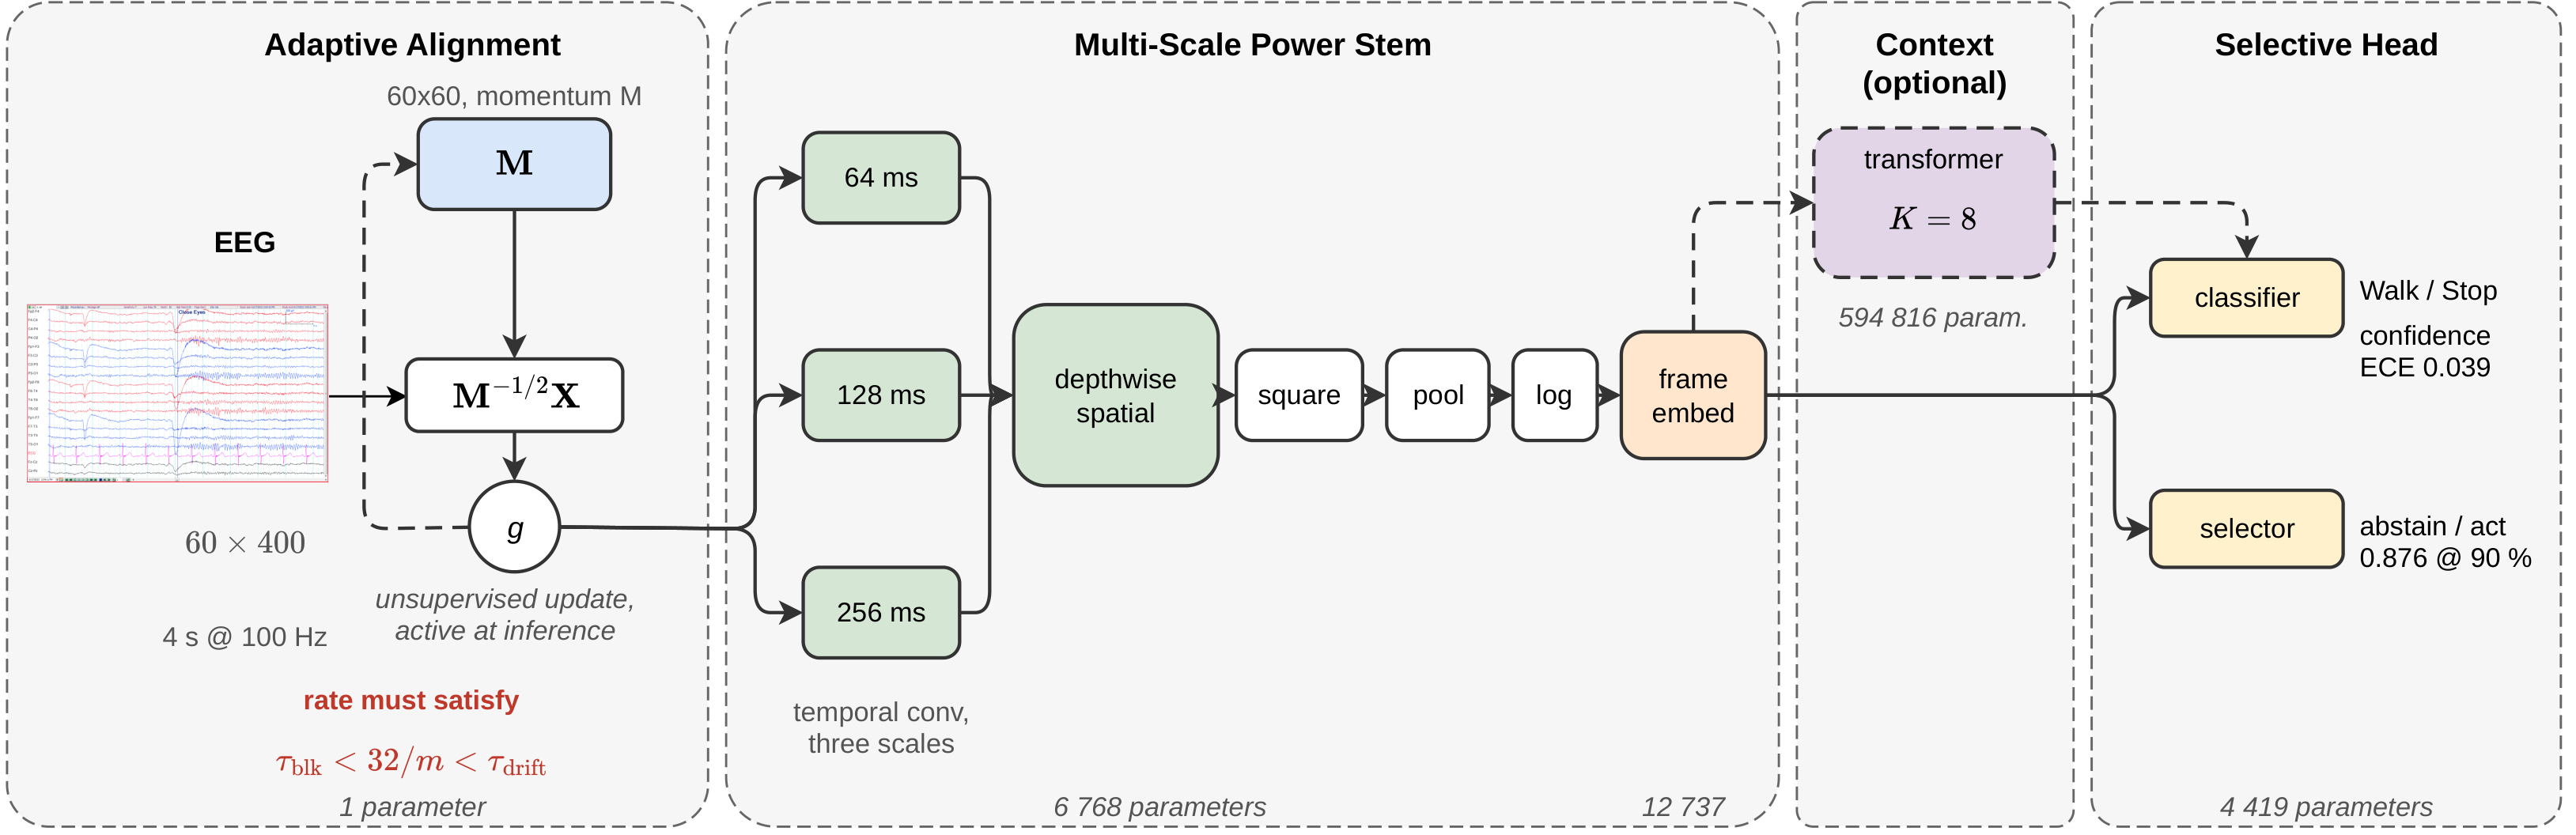
\includegraphics[width=\textwidth]{../results/fig_arch.png}
\caption{The proposed architecture. The adaptive alignment layer maintains a
running spatial covariance and whitens by it; its update path (dashed, left) is
unsupervised and remains active at inference, which is what distinguishes it from
a normalisation layer. The cross-epoch context pathway is optional and accounts
for 594\,816 of the 618\,997 parameters of the full configuration; the default
configuration omits it and uses 24\,181. Parameter counts are exact.}
\label{fig:arch}
\end{figure*}

\subsection{Overview}

The model consumes a window of $C$ channels $\times$ $T$ samples and emits a
class posterior together with a selection score. In its sequence variant it
consumes $K=8$ consecutive epochs at stride 3 (a 14.5\,s span) and predicts the
label of the last epoch; all masks are causal, so only present and past
information is used, which is the only variant a worn device can run.

\subsection{Adaptive Alignment}

The layer maintains a running mean spatial covariance $\mathbf{M}$, applies
$\mathbf{M}^{-1/2}$, and interpolates between the aligned and raw signal through
a learned scalar gate. Two properties distinguish it from a normalisation layer.

First, the update is \textbf{unsupervised}: it uses only the covariance of
incoming windows and therefore runs at inference on unlabelled data. Second, the
estimate updates in \textbf{eval mode}, unlike BatchNorm~\cite{batchnorm}.
Freezing running statistics at test time is correct when train and test share a
distribution; here they are weeks apart, and freezing discards exactly the
adaptation the layer exists to provide.

Each window's covariance is normalised by its own trace before being accumulated:
\begin{equation}
\mathbf{M} \leftarrow (1-m)\,\mathbf{M} + m \cdot
\frac{1}{N}\sum_{n=1}^{N} \frac{\mathbf{C}_n}{\mathrm{tr}(\mathbf{C}_n)/C},
\qquad
\mathbf{C}_n = \frac{\tilde{\mathbf{X}}_n \tilde{\mathbf{X}}_n^{\top}}{T}
\end{equation}
where $\tilde{\mathbf{X}}_n$ is the mean-centred window and $m$ the momentum.
Without the per-window trace normalisation the estimate is power-weighted: on a
cohort whose majority class carries $1.52\times$ the power, the running estimate
converges toward the majority class covariance rather than sitting between the
classes. Section~\ref{sec:rate} shows this correction is necessary but not
sufficient.

\textbf{The layer's output reaches the classifier.} A whitening layer placed
before a normalisation layer invites the objection that the normalisation simply
undoes it. With identical initialisation on held-out windows, stem outputs
computed with and without alignment differ by 36\,\% in relative magnitude and
their correlation structure differs by 0.108.

\subsection{Multi-Scale Power Stem}

Three parallel temporal resolutions (64, 128 and 256\,ms), each with its own
depthwise spatial filters, followed by
$\mathrm{square} \rightarrow \mathrm{pool} \rightarrow \log$. Amplitude
normalisation \textbf{precedes} the squaring so that log-power \emph{ratios}
survive: scaling a window by $s$ shifts its log-power by a constant that a later
affine layer absorbs, whereas normalising after the square destroys the ratio
that event-related desynchronisation~\cite{erd} is expressed in.

This ordering is not cosmetic. In a separate controlled experiment, correcting
the normalisation order was worth $+0.134$ (cohort A) and $+0.174$ (cohort B) on
band-power features, while the same correction applied to a correlation-only
representation --- which carries no marginal power --- moved accuracy by
$+0.000$, a dose--response consistent with the stated mechanism.

\subsection{Causal Cross-Epoch Context}

A causal transformer encoder over the $K$-epoch sequence. Measured state
persistence in cohort A is high: self-transition probability 0.984 (Stop) and
0.955 (Walk) at a 0.5\,s step, corresponding to 12--32\,s dwell times.

\subsection{Selective Head}

A classifier paired with an abstention gate trained under a coverage constraint
following~\cite{selectivenet}, with a full-coverage auxiliary term so that the
backbone continues to learn from every sample rather than only from the covered
region.

%-----------------------------------------------------------------------------
\section{Experimental Setup}

\subsection{Data}

\textbf{Cohort A --- exoskeleton (OpenNeuro ds007788).} 7 subjects $\times$ 9
sessions recorded across weeks; 60-channel active EEG at 100\,Hz; walk/stop
labels from the exoskeleton controller state. Windows of 4\,s at 0.5\,s stride,
approximately 5031 fitting windows per subject. Fitted on sessions 1--3, tested
on sessions 4--9.

\textbf{Cohort B --- treadmill MoBI~\cite{luu}.} 8 subjects $\times$ 3 trials;
64-channel EEG at 100\,Hz; walk/stand from treadmill phase. Fitted on trial 1,
tested on trials 2--3; 2\,s windows. An independent laboratory, different
sensors, a different task framing, and \textbf{reversed class balance} (Stop is
the minority at $\sim$12\,\% here and the majority in cohort A).

The two protocols differ sharply in temporal structure, which
Section~\ref{sec:rate} shows to be decisive:

\begin{table}[htbp]
\caption{Contiguous single-class block structure}
\label{tab:blocks}
\centering
\begin{tabular}{lrrr}
\toprule
Cohort & Blocks & Median length & Longest \\
\midrule
A (exoskeleton) & 109 & 18 windows & 126 \\
B (treadmill)   & 7   & 309 windows & 2211 \\
\bottomrule
\end{tabular}
\end{table}

\subsection{Outcome Measures}

Balanced accuracy for comparability; expected calibration error (ECE), because a
device acting on a confidence value needs it to mean something; accuracy at
90\,\% coverage, the trained selective operating point; spurious activations per
minute of standing; and detection latency, reported alongside the benefit that
buys it.

\textbf{Leakage guard.} Unconditioned nuisance-decodability is confounded with
accuracy --- in our harness a decoder that uses no movement information whatever
measures $R^2 = +0.863$ --- so movement leakage is measured \emph{conditional on
the class label} throughout.

\subsection{Reproducibility and Measurement Noise}
\label{sec:noise}

Two ablation arms disable alignment entirely and therefore never invoke the
running estimator; for them, momentum and estimator version are inert and every
run is a true repeat. These arms measure the noise floor directly
(Table~\ref{tab:noise}).

\begin{table}[htbp]
\caption{Run-to-run spread on arms where the manipulated variable is inert}
\label{tab:noise}
\centering
\begin{tabular}{llrrr}
\toprule
Arm & Transformer & $n$ & Spread & SD \\
\midrule
Stem only, cohort B      & no  & 3 & \textbf{0.0000} & 0.0000 \\
No-align, cohort A       & yes & 3 & 0.0069 & 0.0039 \\
No-align, cohort B       & yes & 4 & 0.0107 & 0.0049 \\
\bottomrule
\end{tabular}
\end{table}

The stem-only arm reproduces its score bit-for-bit across three runs; the arms
containing the cross-epoch transformer do not, and the attention path is the only
structural difference between them. We attribute the variation to
non-deterministic reductions in scaled dot-product attention on GPU.
\textbf{Consequently any arm containing the transformer carries $\approx$0.010
run-to-run noise, and differences below 0.02 in such arms are not interpreted.}
Conversely, an exact null in the deterministic arm is stronger evidence than
``within noise'', because that arm has no noise to hide in.

%-----------------------------------------------------------------------------
\section{Results}

\subsection{Component Ablation, Cohort A}

Table~\ref{tab:ablation} reports the full ablation. All cells use the original
estimator so that the arms are mutually comparable; the per-window correction of
Section~\ref{sec:rate} was measured later and is noted where it applies.

\begin{table}[htbp]
\caption{Component ablation, cohort A, seed 0. Acc@90 is the accuracy at
90\,\% coverage; FA/min is spurious activations per minute of standing.}
\label{tab:ablation}
\centering
\begin{tabular}{llrrrr}
\toprule
Arm & Components & Acc & ECE & Acc@90 & FA/min \\
\midrule
\textbf{Ours}  & align + gate        & \textbf{0.901} & \textbf{0.039} & \textbf{0.876} & 1.64 \\
               & align + ctx + gate  & 0.878 & 0.074 & 0.837 & 1.26 \\
               & align + ctx         & 0.862 & 0.072 & --- & 1.26 \\
               & ctx + gate          & 0.827 & 0.091 & 0.778 & 0.73 \\
               & stem only           & 0.827 & 0.082 & 0.823 & 0.73 \\
\bottomrule
\end{tabular}
\end{table}

\begin{figure*}[t]
\centering
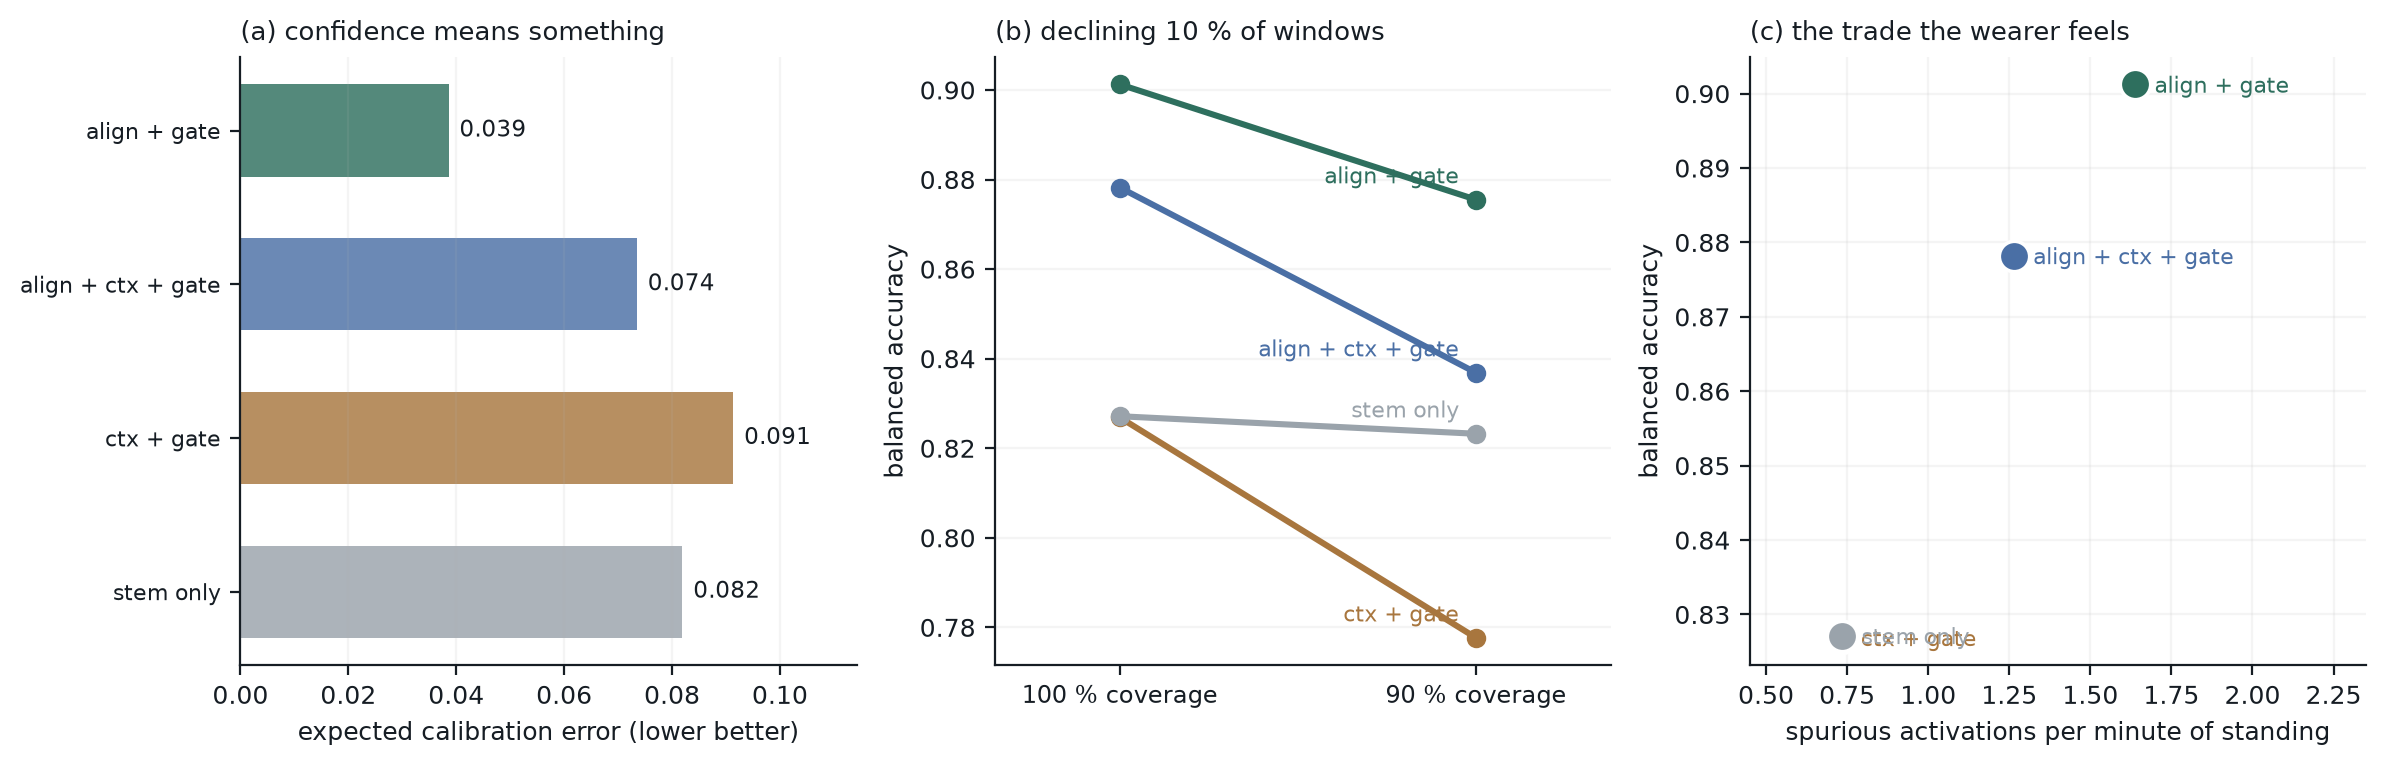
\includegraphics[width=\textwidth]{../results/fig_operating.png}
\caption{Outputs beyond the class label, cohort A. (a) Expected calibration
error by arm: the proposed configuration is the best calibrated, and the arms
without the selective head are the worst. (b) Accuracy recovered by declining the
least-confident 10\,\% of windows. (c) The trade the wearer experiences ---
balanced accuracy against spurious activations per minute of standing.}
\label{fig:operating}
\end{figure*}

\textbf{Alignment is necessary, not additive.} With alignment removed, the
context and gate modules together contribute between 0.000 and 0.007 (the
no-align arm spans 0.827--0.834 across repeats while the stem-only arm is
deterministic at 0.827). Against the 0.010 noise floor of
Section~\ref{sec:noise} that is indistinguishable from nothing, and an order of
magnitude below alignment's own contribution.

\textbf{Cross-epoch context is an operating point, not a default.} Adding it
costs 0.023 accuracy and doubles calibration error, while reducing spurious
activations by 23\,\%. We therefore report it as a selectable safety mode rather
than part of the default configuration --- and note that removing it also removes
594\,816 of the model's 618\,997 parameters, which is what makes the default
configuration compact.

\subsection{Comparison with Published Decoders}

\textbf{A caution on harnesses.} Our architecture and the ATCNet variants were
evaluated in one training harness; the remaining published baselines were
evaluated in an earlier one. ATCNet was run in both and scores 0.913 and 0.881
respectively, so \textbf{the two harnesses differ by 0.032 for an identical
model} --- larger than most of the differences of interest. We therefore report
the two groups separately (Table~\ref{tab:compare}) and do not compare across
them. Doing so would be the single easiest way to manufacture a favourable
result, and the harness offset is reported precisely so that a reader can see it
has not been done here.

\begin{table}[htbp]
\caption{Cohort A comparison. Groups are separated by training harness and must
not be compared across the rule. Parameter counts are exact.}
\label{tab:compare}
\centering
\begin{tabular}{lrr}
\toprule
Model & Params & Balanced acc. \\
\midrule
\multicolumn{3}{l}{\emph{Harness C (this work), seed 0}}\\
ATCNet~\cite{atcnet}                & 45\,280 & \textbf{0.913} \\
ATCNet, rate-matched kernels        & 45\,280 & 0.908 \\
\textbf{Ours, align + gate}         & \textbf{24\,181} & 0.901 \\
Ours, align + ctx + gate            & 618\,997 & 0.878 \\
Ours, stem only                     & 6\,768  & 0.827 \\
\midrule
\multicolumn{3}{l}{\emph{Harness F (earlier), mean of 2 seeds}}\\
ATCNet~\cite{atcnet}                & 45\,280 & 0.879 \\
EEGNeX~\cite{eegnex}                & 58\,082 & 0.876 \\
ShallowFBCSPNet~\cite{schirrmeister}& 97\,120 & 0.867 \\
EEG Conformer~\cite{conformer}      & 440\,706 & 0.843 \\
\bottomrule
\end{tabular}
\end{table}

\begin{figure}[t]
\centering
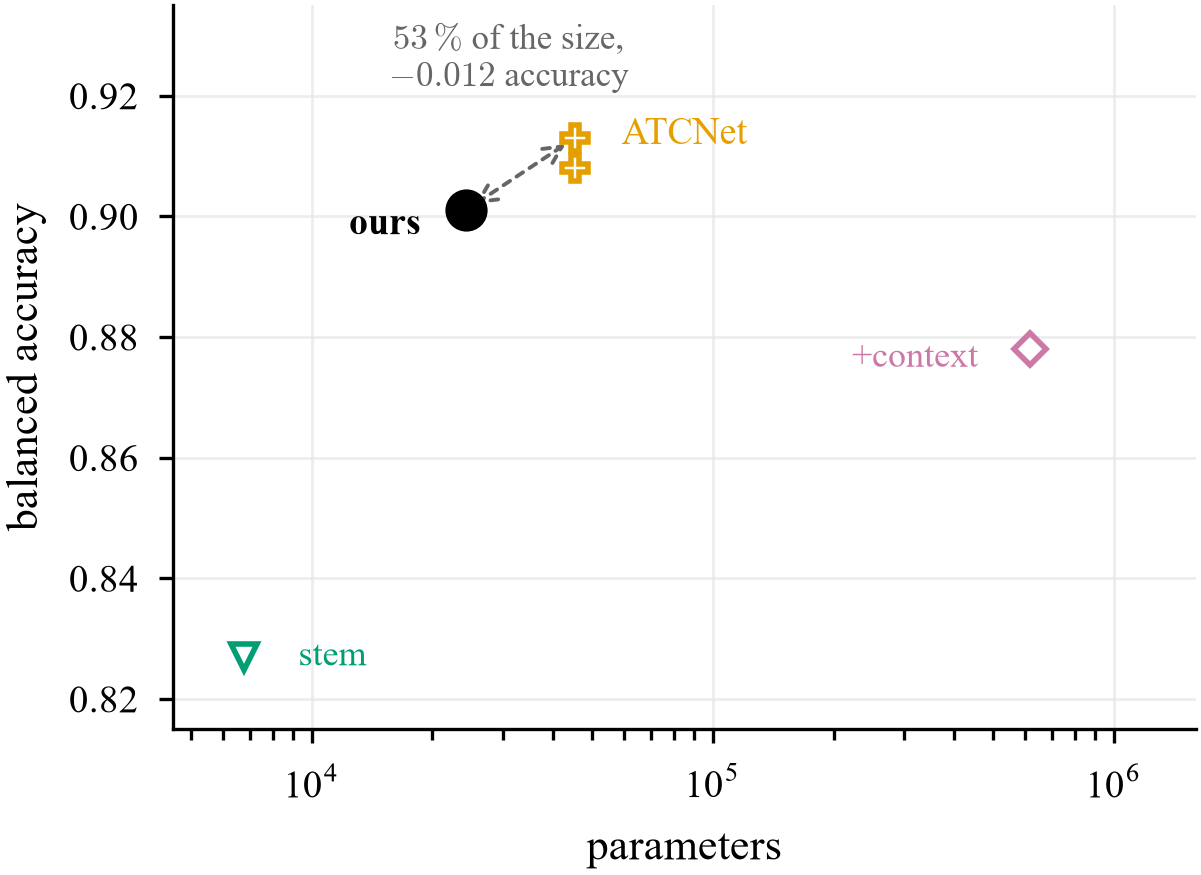
\includegraphics[width=\columnwidth]{../results/fig_efficiency.png}
\caption{Balanced accuracy against parameter count on cohort A, harness C only.
The proposed configuration sits 0.012 below ATCNet at 53\,\% of its parameters.
No point from the other harness appears here.}
\label{fig:efficiency}
\end{figure}

\textbf{We do not claim an accuracy improvement.} In the harness where both were
measured, ATCNet scores 0.913 against our 0.901 --- ATCNet is ahead by 0.012, and
while that is close to the noise floor we report it as a loss rather than a tie.
What our configuration does offer is \textbf{parity at 53\,\% of ATCNet's
parameters and 5\,\% of EEG Conformer's}, together with calibrated confidence
(ECE 0.039) and a trained abstention operating point (0.876 at 90\,\% coverage),
neither of which the baselines provide. Those are the claims we make.

\subsection{The Drift Mechanism}

We measure the affine-invariant Riemannian distance between the fitting-session
mean covariance and each held-out session's, before and after the layer.
Riemannian rather than Frobenius because covariances do not form a vector space
and the Frobenius distance is dominated by scale, which would flatter any
whitening operation.

\begin{table}[htbp]
\caption{Session-drift reduction. The no-op control shares every code path but
never updates its estimate.}
\label{tab:drift}
\centering
\begin{tabular}{lrrrrl}
\toprule
Cohort & $n$ & Raw & Aligned & No-op & Reduction \\
\midrule
A & 7 & 8.372 & 4.082 & 9.173 & $\mathbf{52.0 \pm 4.5\,\%}$ \\
B & 8 & 6.479 & 1.074 & 6.309 & $\mathbf{83.9 \pm 3.9\,\%}$ \\
\bottomrule
\end{tabular}
\end{table}

\begin{figure*}[t]
\centering
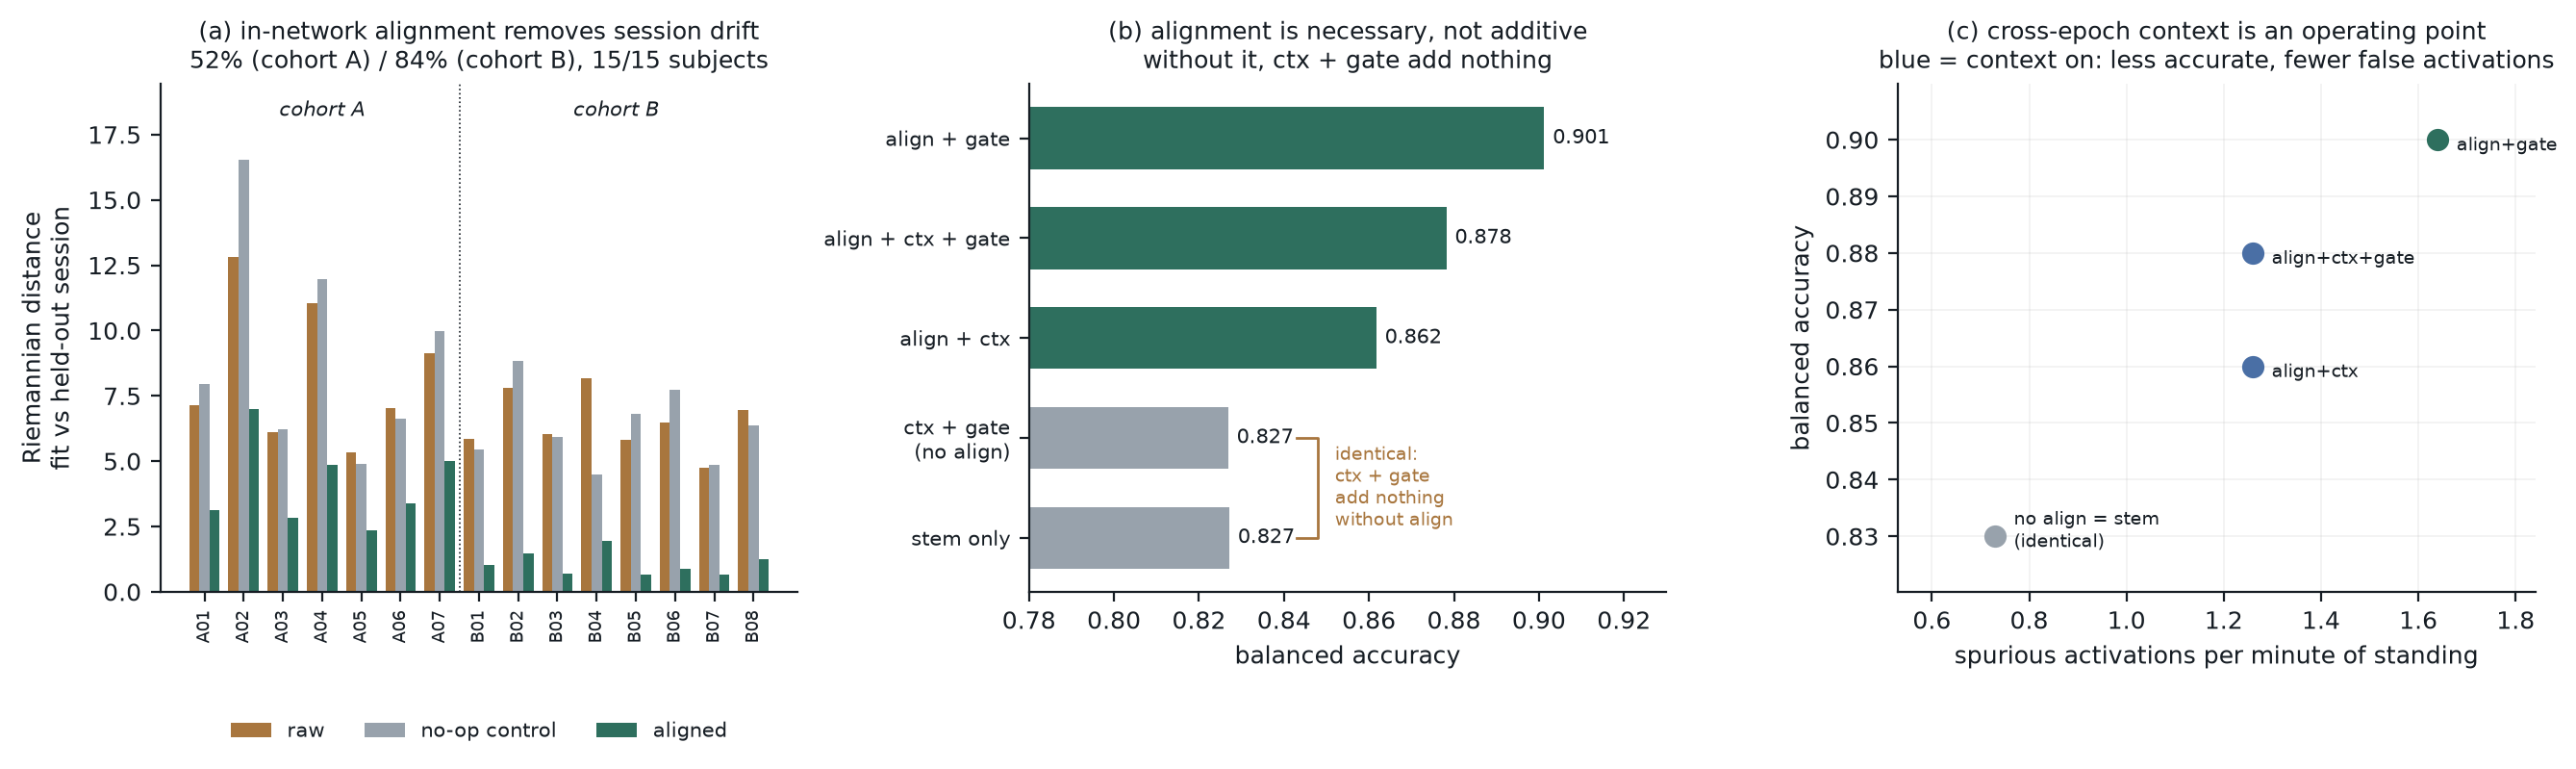
\includegraphics[width=\textwidth]{../results/fig_driftnet.png}
\caption{(a) Riemannian distance between the fitting-session mean covariance and
each held-out session, per subject, for both cohorts, with the momentum-0 no-op
control. Drift falls in every subject; the control shows no reduction.
(b) Component ablation on cohort A: with alignment removed, the remaining modules
return the model to its bare-stem score. (c) Balanced accuracy against spurious
activations per minute of standing, showing the cross-epoch context as a
selectable operating point rather than a failed module.}
\label{fig:drift}
\end{figure*}

Drift is reduced in \textbf{15 of 15 subjects} ($t=-9.14$, $p=10^{-4}$ for cohort
A; $t=-20.59$, $p<10^{-5}$ for cohort B). The no-op control shows no reduction in
either cohort, establishing that the effect comes from adaptation rather than
from the whitening operation or from the measurement.

\subsection{External Validation: the Architecture Does Not Transfer}

\begin{table}[htbp]
\caption{Both cohorts, seed 0. The ordering inverts.}
\label{tab:external}
\centering
\begin{tabular}{llrr}
\toprule
Arm & Components & Cohort A & Cohort B \\
\midrule
Ours & align + gate       & \textbf{0.901} & 0.581 \\
     & align + ctx + gate & 0.878 & 0.626 \\
     & align + ctx        & 0.862 & 0.606 \\
     & ctx + gate         & 0.827 & \textbf{0.792} \\
     & stem only          & 0.827 & 0.737 \\
\bottomrule
\end{tabular}
\end{table}

\begin{figure}[t]
\centering
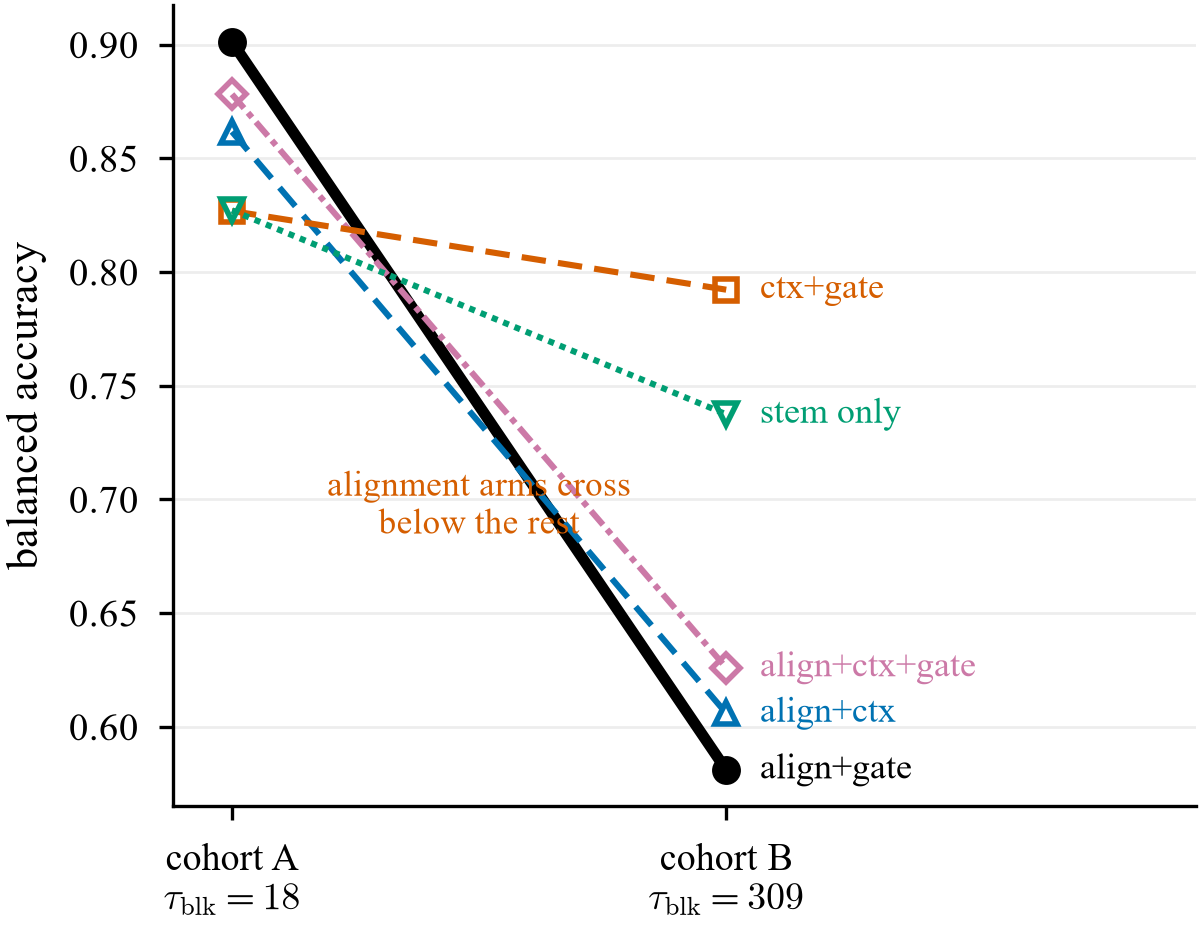
\includegraphics[width=\columnwidth]{../results/fig_inversion.png}
\caption{The same five arms on both cohorts. Solid lines use alignment, dashed
lines do not. The ordering does not compress between cohorts --- it inverts, and
the three alignment arms cross below both alignment-free arms.}
\label{fig:inversion}
\end{figure}

On cohort B the \emph{bare stem} outperforms the full model, 0.737 against 0.626,
and the best cohort-A configuration is the worst cohort-B one. The ordering does
not merely compress; it inverts. We report this in full rather than restricting
the paper to the cohort where the architecture succeeds, and devote the remainder
of the results to explaining it, since the explanation turns out to be the more
useful contribution.

\subsection{The Adaptation Rate Condition}
\label{sec:rate}

\textbf{Diagnosis.} The running estimate tracks whatever is currently streaming.
An exponential moving average with momentum $m$ has an effective memory of
$\approx 1/m$ batches, or $32/m$ windows at our batch size. When a protocol
presents a class in contiguous blocks \emph{longer} than that memory, the
estimate converges to the currently-streaming class and the layer whitens the
class away. Cohort A's blocks (median 18 windows) sit far inside even the fastest
memory; cohort B's (median 309, longest 2211) do not.

\textbf{Prediction.} Slowing adaptation until the memory exceeds a class block
should restore cohort B. Memory is $\approx$160, 640 and 3200 windows at
$m = 0.2$, 0.05 and 0.01.

\begin{table}[htbp]
\caption{Momentum sweep, cohort B, all five arms, seed 0. ``At crossing'' is
$m{=}0.20 \rightarrow 0.05$, where the memory passes the 309-window block.}
\label{tab:sweep}
\centering
\begin{tabular}{lrrrrc}
\toprule
Arm & 0.20 & 0.05 & 0.01 & At crossing & Aligns \\
\midrule
align+ctx+gate & 0.626 & 0.724 & 0.723 & $\mathbf{+0.098}$ & yes \\
align+gate     & 0.581 & 0.671 & 0.696 & $\mathbf{+0.090}$ & yes \\
align+ctx      & 0.606 & 0.700 & 0.726 & $\mathbf{+0.094}$ & yes \\
ctx+gate       & 0.792 & 0.782 & 0.783 & $-0.010$ & \textbf{no} \\
stem only      & 0.737 & 0.737 & 0.737 & $\mathbf{0.000}$ & \textbf{no} \\
\bottomrule
\end{tabular}
\end{table}

Every arm that uses alignment gains 0.090--0.098 as the memory crosses the class
block length. Neither arm that omits alignment responds --- the no-align arm to
within its run-to-run spread, and the stem-only arm \emph{exactly}, reproducing
0.7375 at every setting despite a 160-fold change in adaptation rate. Because
that arm is deterministic (Section~\ref{sec:noise}), this is an exact null rather
than an unresolved one. The manipulated variable therefore acts only through the
component it controls, which an unrelated confound --- optimisation dynamics,
regularisation, run-to-run variance --- would not produce.

\begin{figure*}[t]
\centering
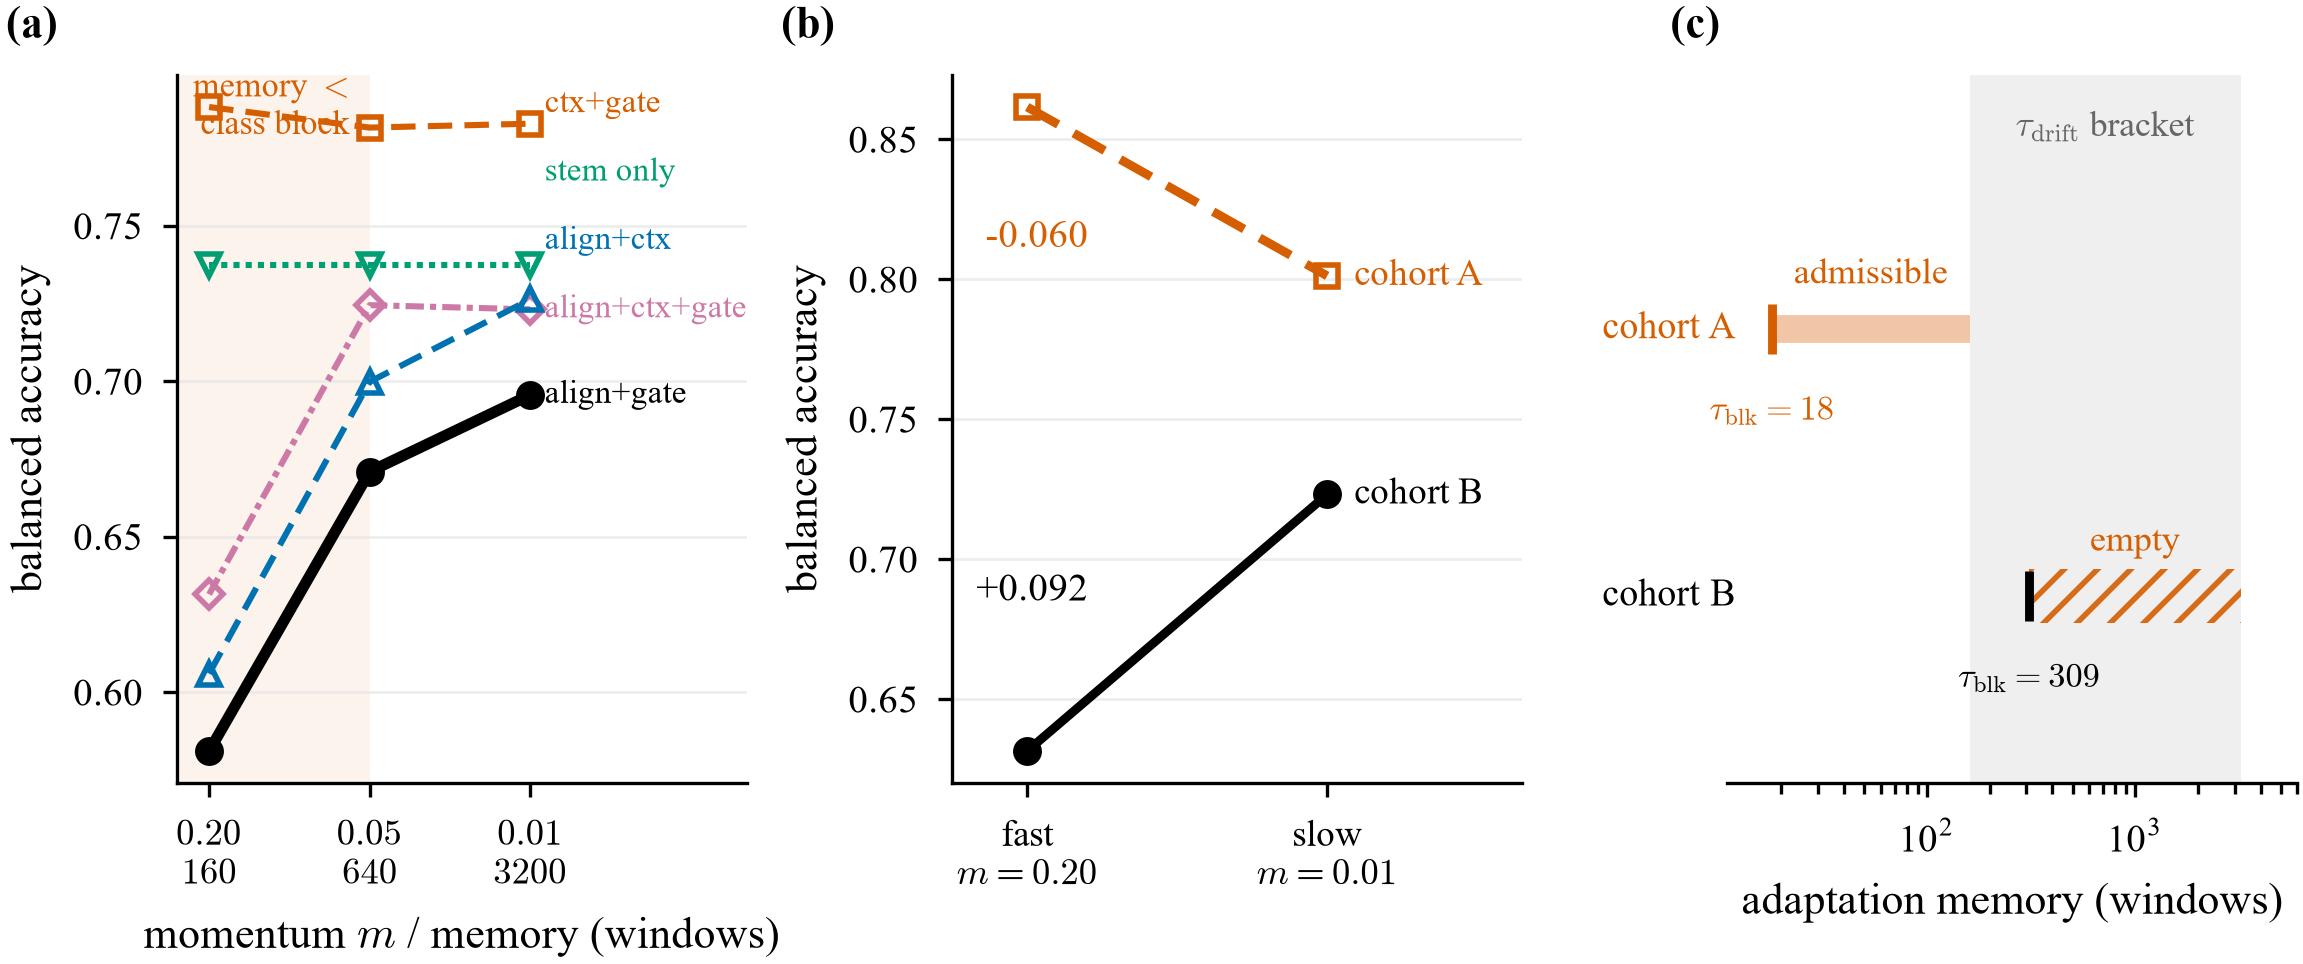
\includegraphics[width=\textwidth]{../results/fig_rate.png}
\caption{The adaptation rate condition. (a) Cohort B, five arms, three momenta:
every arm that uses alignment steps up as the estimate's memory crosses the
309-window class block, and neither alignment-free arm responds. (b) The same
change applied to both cohorts at matched estimator version produces opposite
signs, so no single rate serves both protocols. (c) The admissible band of
(\ref{eq:band}), bounded below by the class-block duration and above by the drift
timescale: wide for cohort A, empty for cohort B.}
\label{fig:rate}
\end{figure*}

\textbf{The condition is two-sided.} We predicted, before running it, that the
same change would be free on cohort A, whose blocks sit far inside even the
fastest memory. It is not
(Table~\ref{tab:twosided}); it costs 0.060.

\begin{table}[htbp]
\caption{The same change applied to both cohorts, matched estimator version.}
\label{tab:twosided}
\centering
\begin{tabular}{lrrr}
\toprule
Cohort & $m=0.20$ & $m=0.01$ & $\Delta$ \\
\midrule
A (blocks 18 win)  & \textbf{0.862} & 0.801 & $\mathbf{-0.060}$ \\
B (blocks 309 win) & 0.631 & \textbf{0.723} & $\mathbf{+0.092}$ \\
\bottomrule
\end{tabular}
\end{table}

The optima are opposite, and error in either direction costs 0.06--0.09. The
rate must be \textbf{fast enough to track drift and slow enough not to track
class}:

\begin{equation}
\tau_{\mathrm{class\text{-}block}} \;<\; \frac{32}{m} \;<\; \tau_{\mathrm{drift}}
\label{eq:band}
\end{equation}

Cohort A satisfies~(\ref{eq:band}) with a wide margin, so fast adaptation is both
safe and useful there. Cohort B's 309-window blocks force the rate slow enough
that it can no longer track drift, so the admissible band is empty. \textbf{This
also explains the residual}: even at its best setting, alignment still costs
0.060 on cohort B, because at the only rate that avoids class-tracking there is
no drift-tracking benefit left to collect. Both $\tau$ in~(\ref{eq:band}) are
properties of the recording protocol and can be computed before a model is
fitted.

This also clarifies why offline Euclidean Alignment~\cite{hewu} does not meet
this failure: a whole-recording estimate is maximally slow, so it never tracks
class --- and never tracks within-recording drift either, which is exactly the
capability an in-network version is introduced to add.

%-----------------------------------------------------------------------------
\section{Discussion}

Domain adaptation and invariance methods are routinely justified by a
distribution-level quantity --- a divergence, an alignment distance, a
nuisance-decodability score --- with task performance assumed to follow. This
work provides five counterexamples within a single system, three of which we
produced by acting on that assumption ourselves.

\begin{enumerate}
\item The adaptation rate was originally selected because it maximised drift
      reduction (60\,\% against 25\,\%). That choice cost 0.092 accuracy on
      cohort B.
\item The cohort where \emph{more} drift was removed (84\,\% against 52\,\%) is
      the cohort where accuracy fell.
\item A verified correction to a genuine covariance-estimation bias moved
      decoding by $+0.005$ and $-0.016$. The mechanism improved; performance did
      not follow.
\item A prediction registered from our own diagnosis was falsified
      (Table~\ref{tab:twosided}), because the diagnosis accounted only for the
      harm the estimate can do and not for the benefit it was delivering.
\item The nuisance-leakage probe rises with accuracy whether or not the decoder
      can access the nuisance ($R^2 = +0.863$ for one that cannot).
\end{enumerate}

\begin{figure}[t]
\centering
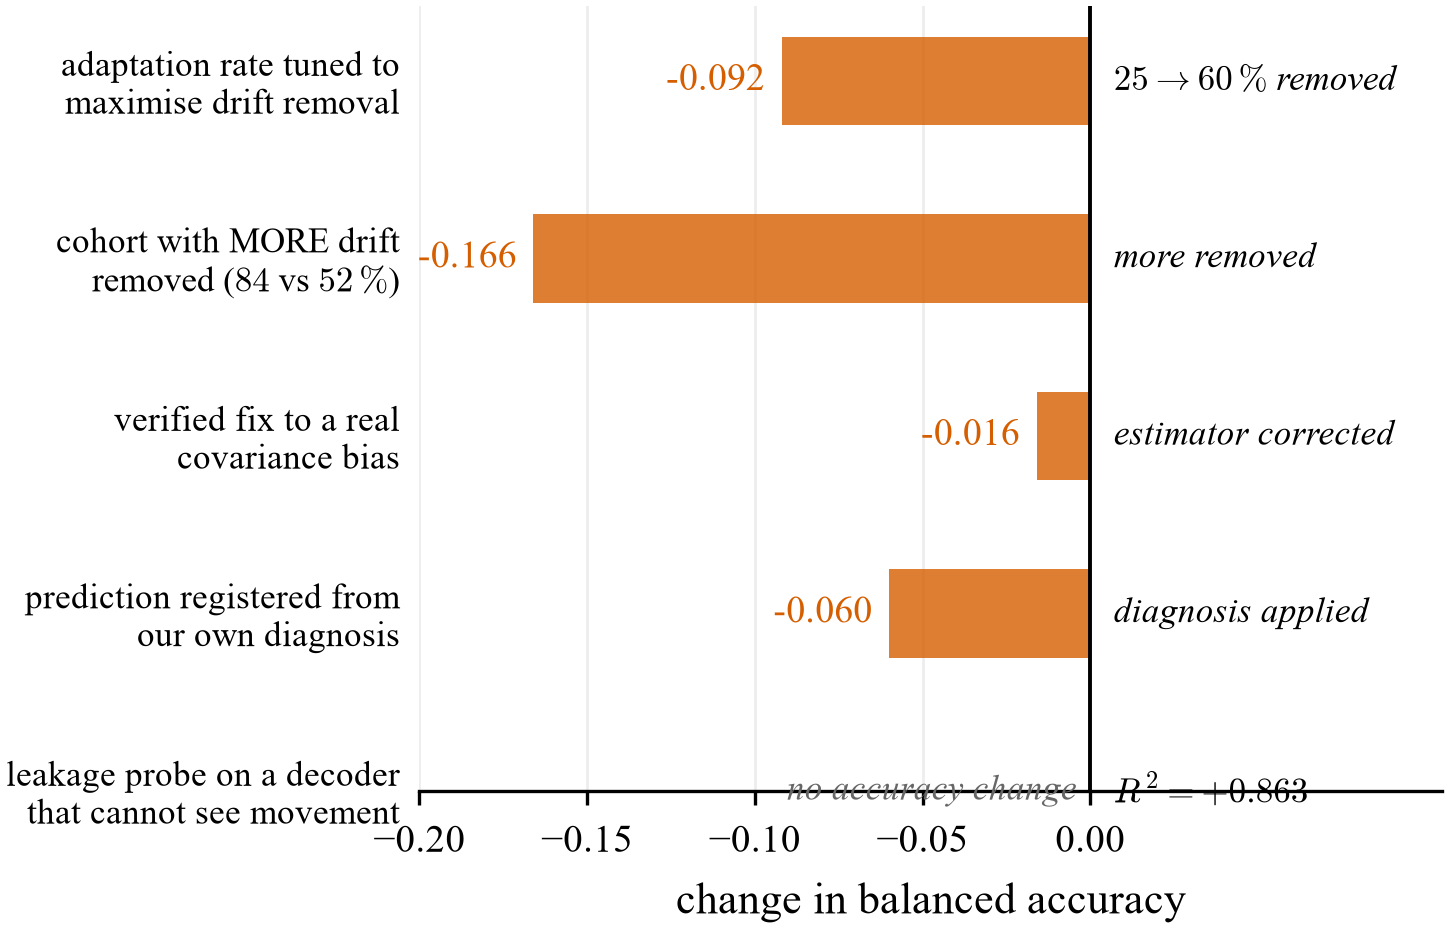
\includegraphics[width=\columnwidth]{../results/fig_metrics.png}
\caption{The five counterexamples. In each row a distribution-level quantity was
improved successfully (right, in green) and the task did not follow (left, in
red). The final row has no accuracy change and therefore no bar: the leakage
probe rises with accuracy whether or not the decoder can access the nuisance.}
\label{fig:metrics}
\end{figure}

Item 4 generalises the rest. Each of these metrics is \textbf{one-sided by
construction}: it scores the failure it was designed to detect and carries no
term for the capability the intervention removes. Drift reduction measures how
much non-stationarity a layer removes and has no term for what the layer
destroys. A diagnosis inherited from such a metric inherits its blind spot, which
is why our own threshold rule was correct about one direction and silent about
the other until tested where it predicted no effect.

\textbf{Limitations.} Ablations are single-seed; with a 0.010 noise floor on
transformer arms, single-seed rankings of closely-spaced models are not
interpretable, and we avoid making them. The two cohorts have 7 and 8 subjects.
Cohort B uses 2\,s windows against cohort A's 4\,s, so the context pathway spans
a shorter duration there. The two-sided account is fitted to two cohorts with
opposite block structure and predicts an interior optimum that we have not
measured; a cohort whose admissible band is narrow but non-empty would test it
properly. Finally, the design rule in~(\ref{eq:band}) was derived after observing
cohort B fail, and although one prediction from it has since been tested
out-of-sample, that test falsified it --- the corrected two-sided form has not
yet predicted anything in advance.

%-----------------------------------------------------------------------------
\section{Conclusion}

We presented a 24\,181-parameter EEG decoder combining label-free in-network
session adaptation, a ratio-preserving multi-scale power stem and a selective
head, reaching 0.901 balanced accuracy with ECE 0.039 and a trained abstention
operating point on a longitudinal exoskeleton cohort, and removing 52--84\,\% of
session-to-session covariance drift across two cohorts in every subject tested.

We do not claim an accuracy improvement: a strong attention baseline scores
0.913 in the same harness. What the work establishes is a condition governing
when in-network adaptation can help at all. An estimate that adapts at test time
tracks whatever is currently streaming, so its rate must exceed the protocol's
class-block timescale and remain below its drift timescale. Where those
requirements cross, no admissible rate exists and the layer should be omitted
rather than tuned. Both quantities are computable from the recording protocol
before any model is fitted, which makes the condition a design-time check rather
than a post-hoc diagnosis.

%-----------------------------------------------------------------------------
\begin{thebibliography}{99}
\bibitem{schirrmeister} R.~T. Schirrmeister \emph{et al.}, ``Deep learning with
convolutional neural networks for EEG decoding and visualization,'' \emph{Human
Brain Mapping}, vol.~38, no.~11, pp.~5391--5420, 2017.

\bibitem{lawhern} V.~J. Lawhern \emph{et al.}, ``EEGNet: a compact convolutional
neural network for EEG-based brain--computer interfaces,'' \emph{J. Neural Eng.},
vol.~15, no.~5, p.~056013, 2018.

\bibitem{eegnex} X.~Chen, X.~Teng, H.~Chen, Y.~Pan, and P.~Geyer, ``Toward
reliable signals decoding for electroencephalogram: a benchmark study to
EEGNeX,'' \emph{Biomed. Signal Process. Control}, vol.~87, p.~105475, 2024.

\bibitem{atcnet} H.~Altaheri, G.~Muhammad, and M.~Alsulaiman,
``Physics-informed attention temporal convolutional network for EEG-based motor
imagery classification,'' \emph{IEEE Trans. Ind. Informat.}, vol.~19, no.~2,
pp.~2249--2258, 2023.

\bibitem{conformer} Y.~Song, Q.~Zheng, B.~Liu, and X.~Gao, ``EEG Conformer:
convolutional transformer for EEG decoding and visualization,'' \emph{IEEE Trans.
Neural Syst. Rehabil. Eng.}, vol.~31, pp.~710--719, 2023.

\bibitem{hewu} H.~He and D.~Wu, ``Transfer learning for brain--computer
interfaces: a Euclidean space data alignment approach,'' \emph{IEEE Trans.
Biomed. Eng.}, vol.~67, no.~2, pp.~399--410, 2020.

\bibitem{barachant} A.~Barachant, S.~Bonnet, M.~Congedo, and C.~Jutten,
``Multiclass brain--computer interface classification by Riemannian geometry,''
\emph{IEEE Trans. Biomed. Eng.}, vol.~59, no.~4, pp.~920--928, 2012.

\bibitem{zanini} P.~Zanini \emph{et al.}, ``Transfer learning: a Riemannian
geometry framework with applications to brain--computer interfaces,'' \emph{IEEE
Trans. Biomed. Eng.}, vol.~65, no.~5, pp.~1107--1116, 2018.

\bibitem{selectivenet} Y.~Geifman and R.~El-Yaniv, ``SelectiveNet: a deep neural
network with an integrated reject option,'' in \emph{Proc. ICML}, 2019,
pp.~2151--2159.

\bibitem{seqsleepnet} H.~Phan \emph{et al.}, ``SeqSleepNet: end-to-end
hierarchical recurrent neural network for sequence-to-sequence automatic sleep
staging,'' \emph{IEEE Trans. Neural Syst. Rehabil. Eng.}, vol.~27, no.~3,
pp.~400--410, 2019.

\bibitem{xsleepnet} H.~Phan \emph{et al.}, ``XSleepNet: multi-view sequential
model for automatic sleep staging,'' \emph{IEEE Trans. Pattern Anal. Mach.
Intell.}, vol.~44, no.~9, pp.~5903--5915, 2021.

\bibitem{batchnorm} S.~Ioffe and C.~Szegedy, ``Batch normalization: accelerating
deep network training by reducing internal covariate shift,'' in \emph{Proc.
ICML}, 2015, pp.~448--456.

\bibitem{erd} G.~Pfurtscheller and F.~H. Lopes da Silva, ``Event-related EEG/MEG
synchronization and desynchronization: basic principles,'' \emph{Clin.
Neurophysiol.}, vol.~110, no.~11, pp.~1842--1857, 1999.

\bibitem{luu} T.~P. Luu, S.~Nakagome, Y.~He, and J.~L. Contreras-Vidal,
``Real-time EEG-based brain--computer interface to a virtual avatar enhances
cortical involvement in human treadmill walking,'' \emph{Sci. Rep.}, vol.~7,
p.~8895, 2017.
\end{thebibliography}

\end{document}
